\section{Evaluation}\label{sec:evaluation} 
In this chapter, I am going to evaluate the outcome of my thesis i.e. research and implementation work. 
Figure~\ref{fig:Evaluation_Phases} shows the phases of the entire evaluation process. Section \ref{subsec:goals} describes the research and case study phase. Section \ref{subsec:designmethod} illustrates the evaluation design method that I have used for conducting the experiment. This is then followed by a brief description of the planning phase in Section \ref{subsec:planning}. Afterward, Section \ref{subsec:execution} describes the preparation and test execution phase in detail. Section \ref{subsec:threats&mitigation} explains the associated threats with the evaluation process and their mitigation criteria. Finally, Section \ref{subsec:results} discusses the results generated from the gathered data. 

The aim of this chapter is as follows: 

"Analyze the outcome of the usage of an interactive demonstrator for the purpose of evaluation with respect to the user from the point of view of the researcher in the context of teaching the basic concepts of bidirectional transformation (bx) and making them understandable and accessible."

\begin{figure}[h]
	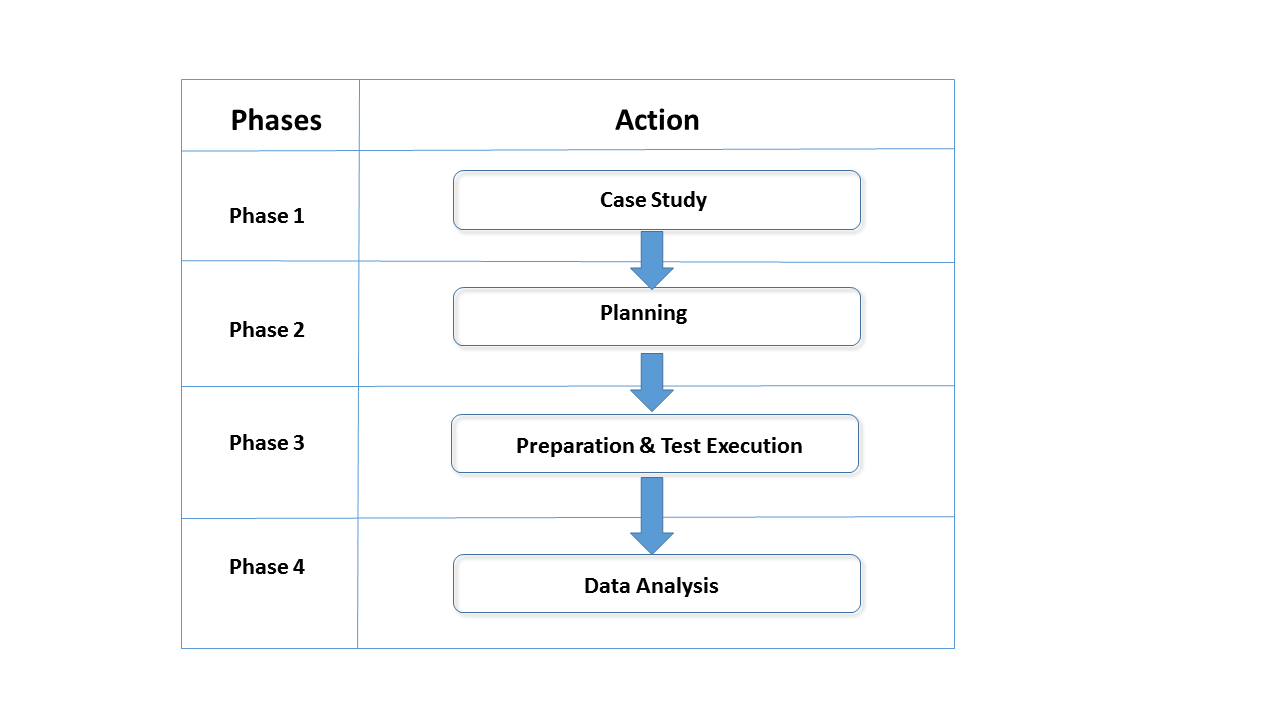
\includegraphics[width=1\textwidth]{figures/Evaluation_Phases}
	\caption{Evaluation Phases}
	\label{fig:Evaluation_Phases}
\end{figure}

\subsection{Goals}\label{subsec:goals}  
In any research, there could be many cases and each case could focus on a number of different research questions, each of which leads to a different direction in developing solution strategies~\cite{semethods}. Hence, for any evaluation process, most important thing are selecting cases that are most relevant to the research and narrowing down the research questions only associated with the exact problems in hand. 

\paragraph{Research Questions}
Our experience based on teaching and cooperation with industry has led us to suspect that people often draw their intuition for desired synchronization behavior directly from the special case of bijections.
This can be problematic and leads to statements such as: ``Why do I need a \emph{bidirectional} transformation language if the transformation at hand is not \emph{bijective}?''
Ironically, bidirectional transformation languages are often especially helpful when a transformation is \emph{not} bijective. As a sub-question of the research question \textbf{RQ 3} described earlier in Section \ref{subsec:contribution}, I propose to investigate if such misconceptions are really widespread or not:

\begin{description}
	\item[RQ 3.1:] Do people tend to derive their (in general wrong) intuition for synchronization scenarios from the special case of bijections?
\end{description}

To impart and train a more general intuition for synchronization scenarios I have implemented \textit{Demon-BX}, an online demonstrator for bidirectional transformations, as a platform for easily creating synchronization scenarios to help achieve corresponding learning goals.
As a proof-of-concept, I have formulated five concrete learning goals and designed corresponding scenarios based on a simple example. I believe (i) that example-based demonstrators are an effective way of achieving my (and similar) learning goals, and (ii) that a demonstrator is only useful in combination with carefully designed scenarios. As a sub-question of the research question \textbf{RQ 4} described earlier in Section \ref{subsec:contribution}, I propose to investigate these conjectures with the following two research questions: 

\begin{description}
	\item[RQ 4.1:] Does demon-bx support achieving the corresponding learning goals?
	\item[RQ 4.2:] How much does this support depend on supplied scenarios?  Would just playing with the demonstrator and the example already have an equal or comparable (positive) effect?
\end{description}

\paragraph{Purpose}
The purpose of the experiment is to evaluate whether it is possible to teach and enhance the understanding of the basic concepts of bx through the demonstrator.

\paragraph{Perspective}
The perspective is from the point of view of the researcher, i.e. the researcher would like to know if the usage of the demonstrator enhances the understanding of bx concepts of a user.

\paragraph{Context}
This experiment is on a bx tool demonstrator which falls under an educational environment and specifically under computer science branch. Hence, this experiment is mainly designed for the group of students/teachers/researchers from computer science area with or without prior knowledge of model driven software development field.

\subsection{Design Method}\label{subsec:designmethod} 
To investigate my research questions, I have used the Pretest-Posttest design method~\cite{analysisprepostdesigns}, a paired data analysis method in which the same experimental object is measured on some variables on two different occasions under different testing conditions. Here, I am using an extension of the Pretest-Posttest design method, called Pretest-Posttest control group design~\cite{expandquasiexpdesign}. It is a popular research design. The design principle is relatively simple and involves two groups, a test group and a control group. First, the groups are pre-tested and then the test group is given the treatment. Afterward, both the groups are post-tested and data is collected from both occasions. Then, the analysis is done by comparing pretest and posttest results collected from both the groups.

Selection of the Pretest-Posttest control group design method for the experiment is driven by the following reasons~\cite{anovapreposttest}:
\begin{itemize}
	\item It provides control over threats to internal validity.
	\item This allows the researchers to collect and compare posttest result from two groups, which give them an idea about the effectiveness of the treatment.
	\item The researcher can see how the groups have performed from pretest to posttest, whether one, both or neither improved over time.
\end{itemize}

In my case, I have designed test questions, one for each learning goal (brief description in Section~ \ref{subsubsec:questions}), to check if a participant has attained the learning goals or not. I am also interested in the participants' subjective level of certainty for every given answer. The experiment is to be conducted as follows:

\begin{enumerate}
	\item All participants are divided randomly into two groups of equal size: the treated group and the control group.
	\item All participants take the pretest (answer all test questions).
	\item Both groups are allowed to use demon-bx for the same amount of time and are provided with an introduction and overview of the concrete example used in the demonstrator.
	The treated group is additionally provided with carefully chosen scenarios to work through, while the control group is not.
	\item When the time is up, all participants take the posttest (answer the same test questions again).
\end{enumerate}

\subsection{Planning}\label{subsec:planning}
This section explains the entire planning phase in detail. In this phase, I have investigated and  finalized all the factors required to evaluate the research questions as well as the execution of the experiment. Following sub-sections describe the factors one by one.

\subsubsection{Participants}\label{subsubsec:participants}
As the context of the experiment is mainly focussed only on the computer science area, it will be conducted on a group of masters' student of computer science branch at Paderborn University. The participants are chosen based on convenience, i.e. the participants are the students taking a similar course.

\subsubsection{Hypotheses}\label{subsubsec:hypotheses}
Formulating hypotheses formally state that what is going to be evaluated in the experiment. I have constructed my hypotheses focussing on the research questions \textbf{RQ 3.1}, \textbf{RQ 4.1}, and  \textbf{RQ 4.2} as described in Section \ref{subsec:goals}. Following are the hypotheses I have chosen to focus on my experiment:\\

\begin{description}
	\item[Operational Hypotheses]
	\item[H$_{OP1}$:] Students have a wrong intuition for and unreasonable expectations of synchronization scenarios (because they derive their intuition from the special case of bijections).
	\item[H$_{OP2}$:] The usage of demon-bx has a positive effect on the achievement of corresponding bx-related learning goals.
	\item[H$_{OP3}$:] Using demon-bx together with suitable scenarios is more effective than without scenarios.
\end{description}

To evaluate the above stated hypotheses, the corresponding null hypotheses are stated below:
\begin{description}
	\item[Null Hypotheses]
	\item[H$_{NU1}$:] Students have a correct intuition for and reasonable expectations for synchronization scenarios.
	\item[H$_{NU2}$:] There is no significant improvement in the learning outcome of the students after using demon-bx.
	\item[H$_{NU3}$:] There is no significant improvement in the learning outcome of the students using demon-bx with suitable scenarios compared to the students using demon-bx without scenarios.

\end{description}

\subsubsection{Experimental Variables}\label{subsubsec:expvariables}
The Hypotheses described above helped in deciding the variables related to the experiment. The following paragraphs describe and Table~\ref{tab:Experimental_Variables} summarizes all of them.

\paragraph{Independent Variables} The independent variables, which the experimenter purposely changes during the experiment are listed below:

\begin{itemize}
	\item Does a group get scenarios to work through or not: nominal (yes or no)
\end{itemize}

\paragraph{Controlled Variables} The controlled variables, which are kept the same throughout the experiment are listed below:

\begin{itemize}
	\item Demonstrator platform: Demon-BX
	\item Concrete example: Planning a kitchen
	\item Group participants are chosen from: \{master students, PhD students, bx researchers, \ldots \}
	\item Test questions: 5
	\item Learning goals: 5
	\item Max. time interval to answer questions: 55 min
\end{itemize}

\begin{table}[h]
	\centering	
	\begin{tabular}{|p{4cm}|p{5cm}|p{6cm}|}
		\hline
		\rowcolor[gray]{.8}	
		\textbf{} & \textbf{Name} & \textbf{Possible Values} \\
		\hline
		Independent Variable & Group gets scenarios to work & nominal (yes or no)\\
		\hline
		Controlled Variables & 
		Demonstrator platform 
		\newline Concrete example
		\newline Group participants
		\newline Test questions
		\newline Learning goals
		\newline Max. time interval	&
		Demon-BX
		\newline Planning a kitchen 
		\newline \{master students, PhD students, \ldots \}
		\newline 5
		\newline 5
		\newline 55 min \\
		\hline	
		Dependent Variables & 
		Correctness score of pretest
		\newline Correctness score of posttest 
		\newline Level of certainty of pretest
		\newline Level of certainty of posttest & 
		ordinal
		\newline ordinal
		\newline interval
		\newline interval \\
		\hline				
		
	\end{tabular}
	\caption{Experimental Variables}
	\label{tab:Experimental_Variables}
\end{table}

\paragraph{Dependent Variables} The dependent variables, which are likely to be changed in response to the independent variable are listed below:

\begin{itemize}
	\item Correctness score of pretest: ordinal
	\item Correctness score of posttest: ordinal
	\item Level of certainty of pretest:  interval
	\item Level of certainty of posttest: interval
\end{itemize}

\subsubsection{Learning Goals \& Questions}\label{subsubsec:questions}
To investigate the research questions \textbf{RQ 3} and its sub-question \textbf{RQ 3.1}, I chose five bx concepts to evaluate the learning goals (referred to as \textbf{LG} from now on) for the experiment. These concepts are related to the fundamentals of bx described as follows:
\begin{description}
	\item[LG 1:] It is possible to avoid/minimize unnecessary information loss in bx.(?)
	\item[LG 2:] Not all possible changes done in one model can be translated/synchronized into another model. (Synchronization is not total)
	\item[LG 3:] Synchronization is interactive. User interaction (or some other, possibly automated means) can be used to decide between multiple equally consistent results (to handle non-determinism: Synchronization is not always functional). 
	\item[LG 4:] Undoing changes in one model to revert to a previous state does not necessarily imply that this can be reflected analogously in the other model. 
	\item[LG 5:] Bx frameworks are not always state based but also can be delta based. The actual change performed can have an effect on synchronization results, even if the final result might appear to be exactly the same in both cases. 
\end{description}

To teach these learning goals, I carefully prepared five scenarios based on the example \textit{Planning a Kitchen} and added to the demonstrator. Each scenario referred to a learning goal. These scenarios involve guidance steps for the user e.g., various actions performed on the user interface in a sequential manner. At the end of the steps, the user learns the corresponding learning goal.

To evaluate these learning goals, I prepared five questions. Each question referred to a concept of bx which also corresponds to a learning goal. The questions are designed to have two sections for answers. One section contains multiple choice answers and the other contains certainty scale ranging from "I just guessed" to "I am certain". Correctness will be decided from the selection of answer in multiple choice section and certainty will be decided from the certainty parameters. Hence, combining the answer and the certainty parameter I can differentiate between \emph{correct answer}, \emph{absolute correct answer}, \emph{wrong answer}, and \emph{absolute wrong answer}. Please refer Appendix for the evaluation test questions.

\subsection{Execution}\label{subsec:execution} 
This section explains the entire experiment execution process in detail along with the preparation steps in the following subsections.

\subsubsection{Preparation }\label{subsubsec:prep}
To handle two separate groups i.e., control and treated and to conduct two separate tests i.e., pretest and posttest on them, I had to prepare well before the experiment date. 

First, I prepared a two-minute video tutorial explaining some of the basic concepts of bx. Then, I prepared a set of questions relating each question to one learning goals and put them into two different forms i.e., pretest and posttest prepared with Google form~\cite{google-forms}. Google form provides a very simple way to prepare a responsive survey form with customized questions which can be shared easily to a mass audience online. Then to investigate the research questions \textbf{RQ 4} and its sub-questions \textbf{RQ 4.1} and \textbf{RQ 4.2}, I prepared the scenarios with the demonstrator to explain the learning goals in a simple way but with a concrete example. Finally, I prepared two different instruction sheets for both the groups explaining the steps they need to follow during the experiment.

\subsubsection{Test Execution}\label{subsubsec:execution}
The experiment was performed on a group of Master students attending a computer science lecture at Paderborn University. They were informed in advance that such experiment will be conducted on a particular date and that their participation in the experiment is completely voluntary with no consequences what so ever. Participants were requested to bring their laptops to the lecture on the day of the experiment.

\paragraph{Confidentiality} The participants were informed regarding the confidentiality and anonymity of data. The purpose of evaluating the tool was stated, but not the hypotheses of the experiment.

\paragraph{Randomization} To perform the experiment, the students were given the instruction sheet prepared earlier for either the control or the treated group randomly while entering the room. The participants were not informed about which group they are in and received suitable and separate instructions for each group.

\paragraph{No Interference} After that, they were asked to sit in two different areas according to their group allotment. The groups were spatially separated so that discussion between groups was almost impossible.

These information sheets had all the appropriate links to the corresponding questionnaires with questions for the pretest and posttest, demonstrator links with prepared scenarios for the treated group, and a different demonstrator link without scenarios for the control group.

Firstly, all participants went through a two-minute video tutorial to establish basic concepts and notation used in the test questions. Then all participants were asked to take the pretest. After finishing the pretest, the students were asked to use the demonstrator links given to them and to work with it. The link given to the control group only had information on how to operate the demonstrator, while the treated group had access to scenarios chosen to support my learning goals. 

After playing with the demonstrator, both groups were asked to take the posttest. Posttest questions were exactly the same as pretest questions but include some extra questions to get additional qualitative feedback about the demonstrator. The experiment was stopped exactly after 55 minutes.

\subsubsection{Data Validation}\label{subsubsec:datavalidation}
Data were collected from 40 students. I stopped taking responses on Google forms i.e. pretest and posttest forms from students exactly after 55 minutes. After the experiment, I checked the data entered by students in both the forms. Data from one student was removed, due to the fact that the data was regarded as invalid as the student could not finish both the test in the given time limit.

Hence, after removing one student out of the 40, I had data from 39 students for statistical analysis and interpretation of the results. Out of 39 students, 21 students were from the control group and remaining 18 were from treated group.

Finally, based on unique identifiers (identifying the group and participant uniquely) derived for each participant, answers from pretest and posttest were evaluated to get the results. 

\subsection{Threats to Validity and Mitigation}\label{subsec:threats&mitigation}
In my evaluation, I have focused on the validity analysis and threats given by Wohlin et al~\cite{expinse} and further explained by Feldt et al~\cite{validitythreatsinse}. 

This section describes all the threats that are associated with the entire evaluation process i.e., planning, preparation, and execution in the following subsections.
 
\subsubsection{Internal Validity}\label{subsubsec:internalvalidity}
\emph{Did the treatment/change I introduced cause the effect on the outcome? Can other factors also have had an effect?}

\medskip
\noindent To measure improvement I am forced to perform arithmetic with ordinal values.
This might be problematic as the difficulty of the test questions might not be equal. If, for example, one of the test questions is much more difficult than all the rest, then subtracting test scores and comparing improvements between groups is questionable. It can be possible that my test questions might not actually be suitable for checking if my learning goals have been reached and thus measuring the output from the test questions does not make any sense. Also, the students being generally unused to and confused by the notation used, it might be possible that they don't even understand the questions and thus cannot improve anything. To avoid these threats, I have carefully prepared the questions corresponding each one of them to a learning goal and tried to ensure that the difficulty level of all the questions is more or less the same. To make the notations more understandable, I have provided extra information about the notation used in the test questions in the two-minute video tutorial shown to all participants before the pretest along with basic bx concepts.

\emph{Do the groups (control and treated) involved in the experiment equally balanced to have a positive effect on the outcome I measure?}

\medskip
\noindent It might be possible that students of equal caliber are sitting together or might have a discussion between the test to have a negative effect on the results. Hence, to avoid that, I have randomly selected students for control and treated group by giving them instruction sheets randomly while entering the class and making them sit in two separate groups apart from each other.

\emph{Does the formula I used for the result calculation produce statistically significant data? Can I draw conclusions based on the data?}

\medskip
\noindent It can be possible that the formula that I have used to calculate the result of the pretest or the posttest taking correctness and certainty into account or the improvement of the posttest compared to the pretest might not produce the exact significant data for further statistical analysis and thus can affect the final outcome. For example, now I am subtracting the pretest result from the posttest result and then dividing it by two for normalization to calculate the improvement. But, there might be other ways to define what improvement is relative to the pretest result. For example, a student might have already improved the maximum he/she could have from pretest to posttest, but dividing it by two for normalization could lower down the actual improvement percentage.

\subsubsection{External Validity}\label{subsubsec:externalvalidity}
\emph{Is the cause and effect relationship I have shown valid in other situations?}

\medskip
\noindent Our results are only valid for the choice of control variables.
This can be problematic as, for example, my test questions might not actually be suitable for checking if my learning goals have been reached.

\emph{Does the treatment/change I introduced have a statistically significant effect on the outcome I measure?}

\medskip
\noindent A problem could be that participants just guess the answers wildly. So it might possible that the data could be faked or incorrect due to mistakes. To avoid faking of data and to add more authenticity to the experiment, I have added certainty values for each question so that I will get to know whether the participant is just guessing the answer or certain about it. Also, I have scrambled the order of the scenarios given to the treated group to play with and the questions asked so that participants will not get a clue about the relation between them.

\subsection{Data Analysis, Results, and Discussion}\label{subsec:results}
To get the results of my experiment, I have investigated each hypothesis with the data collected separately. Analysis of the data and descriptive statistics are used to visualize the collected data. 

In my experiment, I have asked five questions referring to five learning goals. Each question is prepared to test whether a student understood the related bx concept i.e., learning goal or not. As one of the goals of my thesis is to teach bx concepts through the demonstrator and all of my hypotheses are based on the measurement of correctness and improvement of the answers given by the students, I decided to track these variables question wise rather than evaluating the data collectively for all questions.

The formula for result calculation and analysis of each hypothesis is described in the following subsections.

\subsubsection{Formula Used}\label{subsubsec:evaluation_formula}
For statistical analysis of the data collected in two separate groups i.e., control and treated, the formulas I used for the calculation of results for all hypotheses are described below:

For ith Question \textit{Q$_{i}$} and group \textit{X} (where X $\in$ \{control(c), treated(t), combined(com)\}),

\textit{CO$_{pre(X_i)}$} $\in$ \{-1, 1\}, correctness of the answer to the ith pretest question for X group is either 1 ("right") or -1 ("wrong").

\textit{CE$_{pre(X_i)}$} $\in$ [0, 1], certainty of the answer to the ith pretest question for X group is between 0 ("I just guessed") to 1 ("I am certain").

\textit{CO$_{post(X_i)}$} $\in$ \{-1, 1\}, correctness of the answer to the ith posttest question for X group is either 1 ("right") or -1  ("wrong").

\textit{CE$_{post(X_i)}$} $\in$ [0, 1], certainty of the answer to the ith posttest question for X group is between 0 ("I just guessed") to 1 ("I am certain").

\textit{RES$_{pre(X_i)}$} := \textit{CO$_{pre(X_i)}$} $\times$ \textit{CE$_{pre(X_i)}$} $\in$ [-1,  1], result for the ith pretest question for X group is between -1 ("absolutely wrong") to 1 ("absolutely right").

\textit{RES$_{post(X_i)}$} := \textit{CO$_{post(X_i)}$} $\times$ \textit{CE$_{post(X_i)}$} $\in$ [-1,  1], result for the ith posttest question for X group is between -1 ("absolutely wrong") to 1 ("absolutely right").

\textit{IMP$_{(X_i)}$} := (\textit{RES$_{post(X_i)}$} - \textit{RES$_{pre(X_i)}$})/2 $\in$ [-1,  1], improvement for the ith question for X group from pretest to posttest is between -1 ("absolute negative learning") to 1 ("absolute positive learning").

It is important to understand the following points from the above formulas:
\begin{itemize}
	\item while answering any question, being "absolutely wrong" (\textit{RES$_{pre/post(X_i)}$} = -1) is worse than just being "wrong" (\textit{CO$_{pre/post(X_i)}$} = -1) as being absolutely certain about a wrong answer is more harmful than just being wrong.
	\item similarly while answering any question, being "absolutely right" (\textit{RES$_{pre/post(X_i)}$} = 1) is better than just being "right" (\textit{CO$_{pre/post(X_i)}$} = 1) as being absolutely certain about a right answer is more helpful than just being right.
\end{itemize} 

\subsubsection{Analyzing Hypothesis 1}\label{subsubsec:hypothesis1}
Hypothesis 1 i.e., \textbf{H$_{OP1}$} and \textbf{H$_{NU1}$} is designed to investigate research question \textbf{RQ 3.1}. This hypothesis deals with the fact whether students have a wrong intuition for synchronization scenarios. Data for \textbf{RQ 3.1} can be collected from all pretest results, i.e., combining the pretest results from both control and treated group (\textit{RES$_{pre(com_i)}$}). Because at the end of the pre-test, both control and treated group have gone through the same two-minute video tutorial to establish basic concepts, answered the same set of questions, and hence are equally weighted in terms of bx knowledge acquired.

As five questions were asked, the result can be calculated for each question from the pretest data. 

\begin{figure}[h]
	\centering
	\begin{minipage}{.5\textwidth}
		\centering
		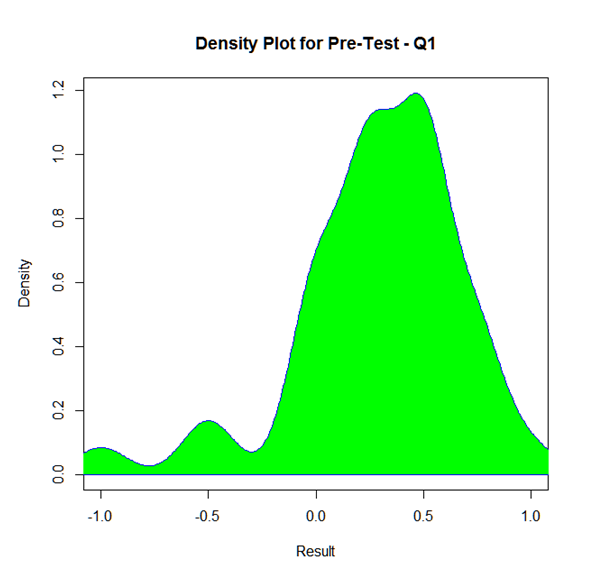
\includegraphics[width=1\linewidth]{figures/Pretest_q1}
		\caption{RES$_{pre(com_1)}$}
		\label{fig:Pretest_q1}
	\end{minipage}%
	\begin{minipage}{.5\textwidth}
		\centering
		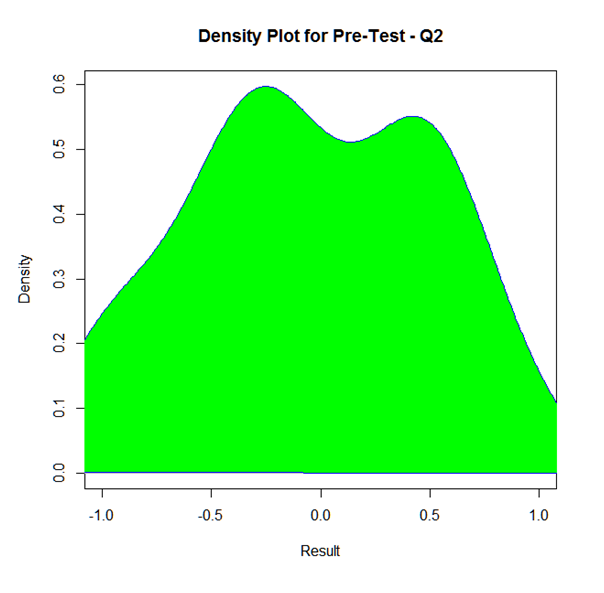
\includegraphics[width=1\linewidth]{figures/Pretest_q2}
		\caption{RES$_{pre(com_2)}$}
		\label{fig:Pretest_q2}
	\end{minipage}
\end{figure}

\begin{figure}
	\centering
	\begin{minipage}{.5\textwidth}
		\centering
		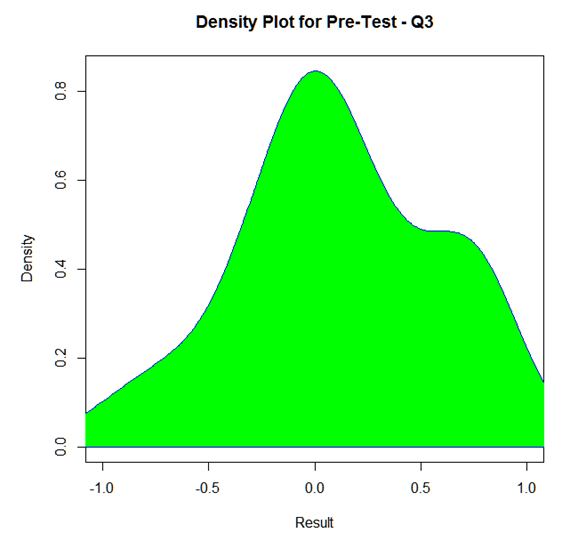
\includegraphics[width=1\linewidth]{figures/Pretest_q3}
		\caption{RES$_{pre(com_3)}$}
		\label{fig:Pretest_q3}
	\end{minipage}%
	\begin{minipage}{.5\textwidth}
		\centering
		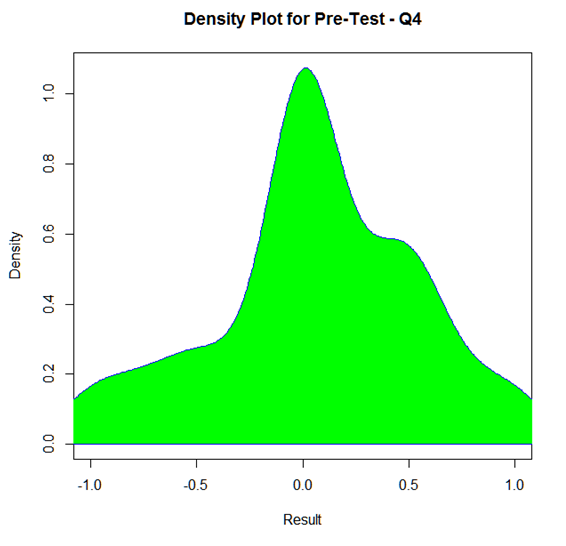
\includegraphics[width=1\linewidth]{figures/Pretest_q4}
		\caption{RES$_{pre(com_4)}$}
		\label{fig:Pretest_q4}
	\end{minipage}
\end{figure}
\begin{figure}
	\centering
	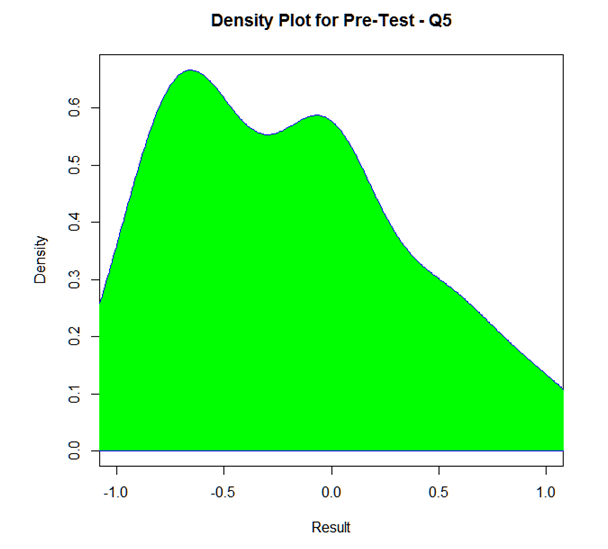
\includegraphics[width=0.5\textwidth]{figures/Pretest_q5}
	\caption{RES$_{pre(com_5)}$}
	\label{fig:Pretest_q5}
\end{figure}

\paragraph{Data Analysis}
After calculating the results i.e., \textit{RES$_{pre(com_i)}$} for each question, I used density plots to show their distribution. Figures~\ref{fig:Pretest_q1}, \ref{fig:Pretest_q2}, \ref{fig:Pretest_q3}, \ref{fig:Pretest_q4}, and \ref{fig:Pretest_q5} show the density plots of the results for each question. In the plots, the x-axis represents the result calculated from combining both correctness and certainty as described in Section \ref{subsubsec:evaluation_formula} ranging between -1 (absolutely wrong) to 1 (absolutely right). The y-axis represents the density of 39 students lying over the interval. From Figure~\ref{fig:Pretest_q1}, it is possible to see that the distribution of the results is mainly on the positive side i.e., between 0 to 1 for Q1. But for all other questions, the distribution of the results is rather scattered over the interval and does not give any conclusive result to accept or reject the null hypothesis just by looking at these plots.

To gain a better understanding of the data, I have further analyzed it with a t-test. As this hypothesis is related to only one set of pretest data, I have used the one-sample t-test.   

As mentioned earlier, certainty value is also involved in the result calculation. Its value entered by the students ranges from 1 ("I just guessed") to 5 ("I am certain") which corresponds to the interval 0 to 1 considered for calculation. Hence, the result of a correct answer with the lowest non-zero certainty value to any question is 0.25. So this hypothesis can be expressed as:   

Null Hypothesis, {H$_{NU1}$}: Mean (\textit{RES$_{pre(com_i)}$}) > 0.25 

Hence, I have included the options (\textit{alternative="less", mu=0.25}) during the calculation which signifies that according to the operational hypothesis the mean value has to be less than 0.25. The results from the t-test are shown in Table~\ref{tab:t-test_PreTest}. The 95\% confidence interval has been included for this t-test.

\paragraph{Discussion}
From the t-test results as shown in Table~\ref{tab:t-test_PreTest}, it can be clearly seen that the mean value of \textit{RES$_{pre(com_i)}$} for question Q1 is just slightly higher than 0.25 and for questions Q2, Q3, Q4, and Q5 is much less than 0.25. Also, the p-values in these cases are very low so the results are highly significant. Most students were just guessing in the pretest.  A few questions were answered correctly but considering the very low certainty values, this does not mean much or imply any deep understanding. However, the increase in the mean value for the question Q1 (refer evaluation test questions in Appendix) is most likely due to the fact that this is the easiest question among all and relatively more participants were able to answer it correctly.

These results reject the null hypothesis {H$_{NU1}$}. This indicates that the students derive their (in general wrong) intuition for and expectations of synchronization scenarios from the special case of bijections. Hence, there is indeed a need to teach correct expectations for synchronization scenarios and a demonstrator can be potentially very useful in spreading bx concepts.

\begin{table}[ht]
	\centering	
	\begin{tabular}{|p{1cm}|p{1.5cm}|p{4cm}|p{1.5cm}|p{1.5cm}|p{1.5cm}|}
		\hline
		\rowcolor[gray]{.8}	
		\textbf{} & \textbf{Students} & \textbf{Factor} & \textbf{t-value} & \textbf{p-value} & \textbf{mean}\\
		\hline
		Q1 & 39 & pre test result & 0.7293 & 0.7649 & 0.2948\\
		\hline
		Q2 & 39 & pre test result & -3.3139 & 0.0010 & -0.0448\\
		\hline
		Q3 & 39 & pre test result & -1.8514 & 0.0359 & 0.1089\\
		\hline	
		Q4 & 39 & pre test result & -2.3902 & 0.0109 & 0.0641\\
		\hline
		Q5 & 39 & pre test result & -5.0889 & 0.000005 & -0.1987\\
		\hline			
	\end{tabular}
	\caption{t-test showing Result for Pre-Test (All Participants)}
	\label{tab:t-test_PreTest}
\end{table}

\subsubsection{Analyzing Hypothesis 2}\label{subsubsec:hypothesis2}
Hypothesis 2 i.e., \textbf{H$_{OP2}$} and \textbf{H$_{NU2}$} is designed to investigate research question \textbf{RQ 4.1}. This hypothesis deals with the fact whether demon-bx tool has a positive effect on the achievement of corresponding bx-related learning goals. Data for \textbf{RQ 4.1} can be collected from the improvement calculated for the control group (\textit{IMP$_{(c_i)}$}) and the treated group (\textit{IMP$_{(t_i)}$}) separately. Because both control and treated group have used demon-bx tool (with different environments) before posttest and improvement indicates how much a certain group has improved/learned from pretest to posttest. 

As five questions were asked, the improvement can be calculated for each question from the pretest and the posttest data separately for control and treated group. 

\begin{figure}
	\centering
	\begin{minipage}{.5\textwidth}
		\centering
		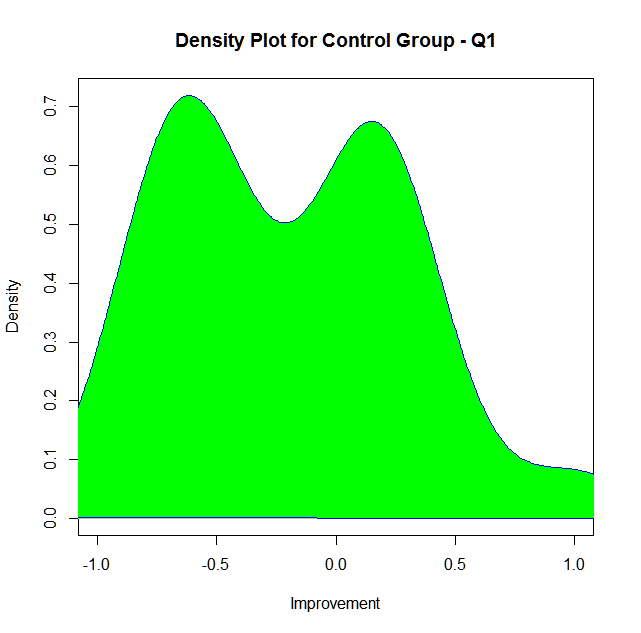
\includegraphics[width=1\linewidth]{figures/Imp_Control-q1}
		\caption{IMP$_{(c_1)}$}
		\label{fig:Imp_Control-q1}
	\end{minipage}%
	\begin{minipage}{.5\textwidth}
		\centering
		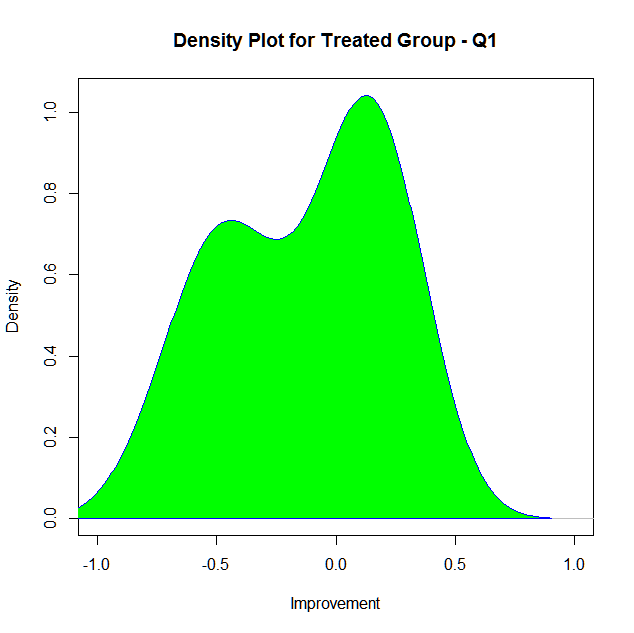
\includegraphics[width=1\linewidth]{figures/Imp_Treated-q1}
		\caption{IMP$_{(t_1)}$}
		\label{fig:Imp_Treated-q1}
	\end{minipage}
\end{figure}

\begin{figure}
	\centering
	\begin{minipage}{.5\textwidth}
		\centering
		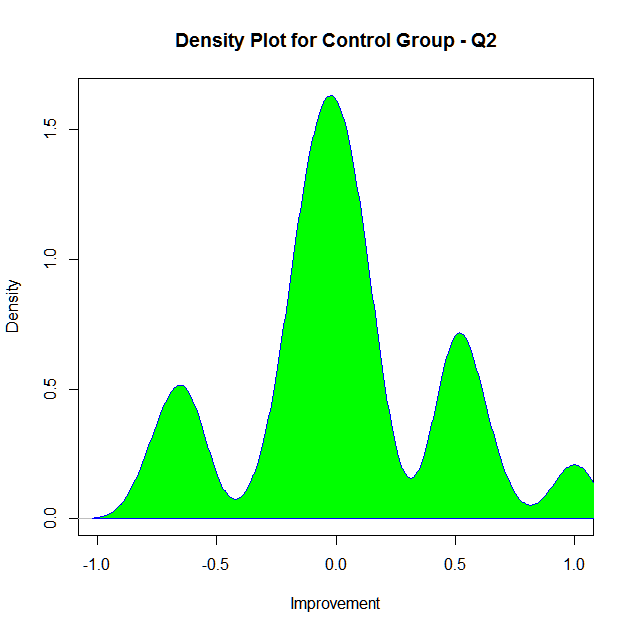
\includegraphics[width=1\linewidth]{figures/Imp_Control-q2}
		\caption{IMP$_{(c_2)}$}
		\label{fig:Imp_Control-q2}
	\end{minipage}%
	\begin{minipage}{.5\textwidth}
		\centering
		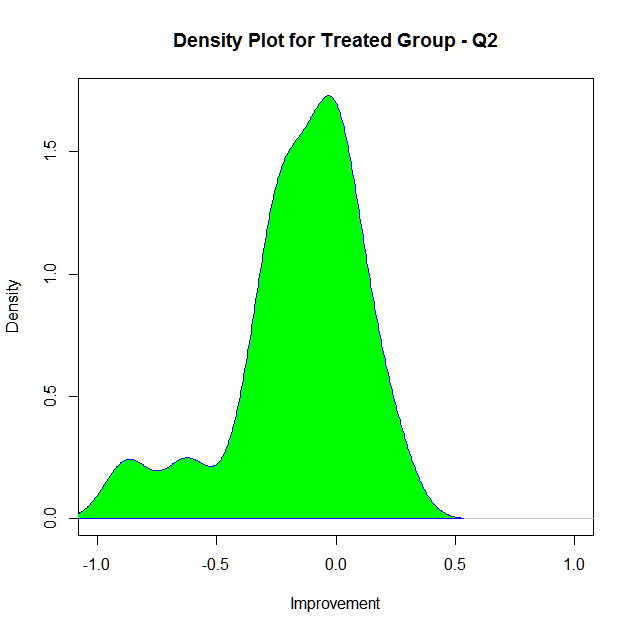
\includegraphics[width=1\linewidth]{figures/Imp_Treated-q2}
		\caption{IMP$_{(t_2)}$}
		\label{fig:Imp_Treated-q2}
	\end{minipage}
\end{figure}

\begin{figure}
	\centering
	\begin{minipage}{.5\textwidth}
		\centering
		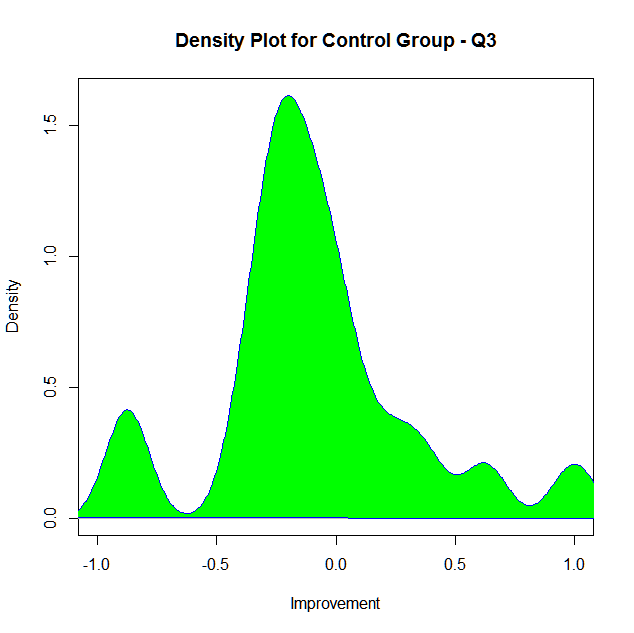
\includegraphics[width=1\linewidth]{figures/Imp_Control-q3}
		\caption{IMP$_{(c_3)}$}
		\label{fig:Imp_Control-q3}
	\end{minipage}%
	\begin{minipage}{.5\textwidth}
		\centering
		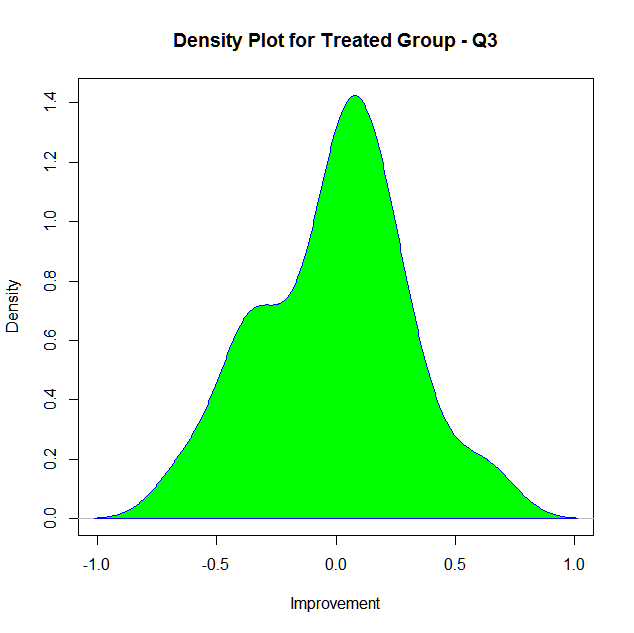
\includegraphics[width=1\linewidth]{figures/Imp_Treated-q3}
		\caption{IMP$_{(t_3)}$}
		\label{fig:Imp_Treated-q3}
	\end{minipage}
\end{figure}

\begin{figure}
	\centering
	\begin{minipage}{.5\textwidth}
		\centering
		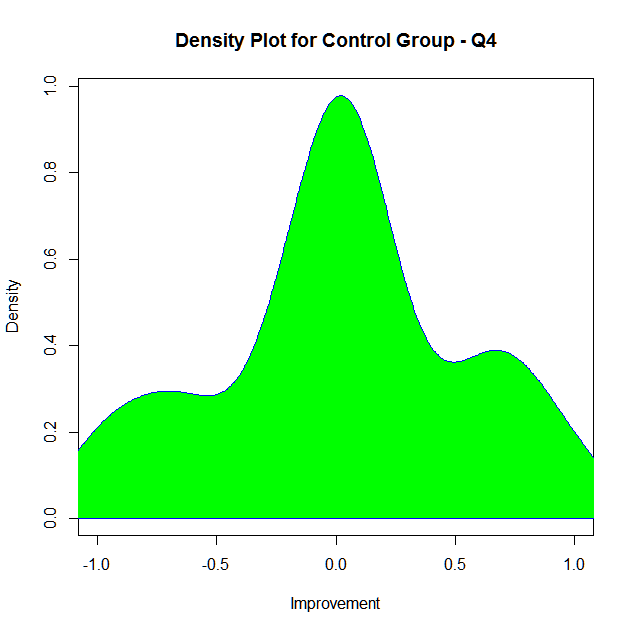
\includegraphics[width=1\linewidth]{figures/Imp_Control-q4}
		\caption{IMP$_{(c_4)}$}
		\label{fig:Imp_Control-q4}
	\end{minipage}%
	\begin{minipage}{.5\textwidth}
		\centering
		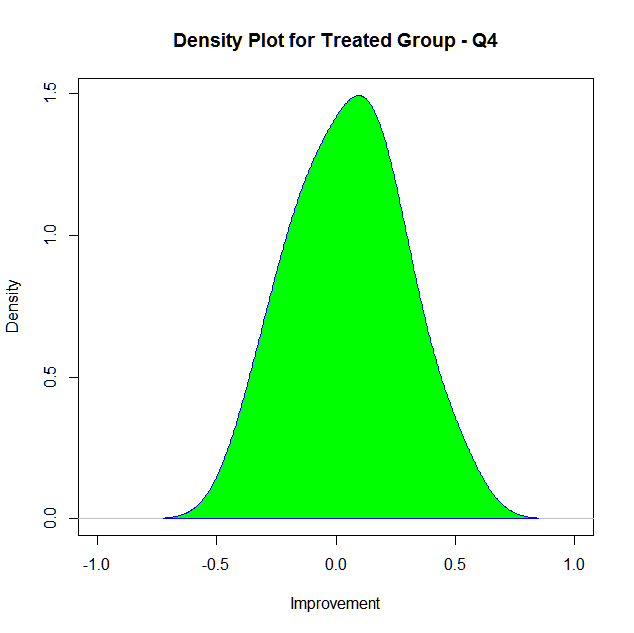
\includegraphics[width=1\linewidth]{figures/Imp_Treated-q4}
		\caption{IMP$_{(t_4)}$}
		\label{fig:Imp_Treated-q4}
	\end{minipage}
\end{figure}

\begin{figure}
	\centering
	\begin{minipage}{.5\textwidth}
		\centering
		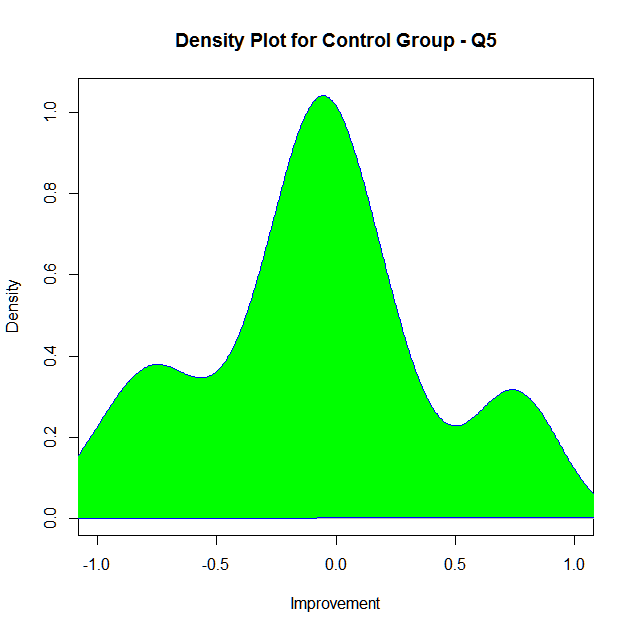
\includegraphics[width=1\linewidth]{figures/Imp_Control-q5}
		\caption{IMP$_{(c_5)}$}
		\label{fig:Imp_Control-q5}
	\end{minipage}%
	\begin{minipage}{.5\textwidth}
		\centering
		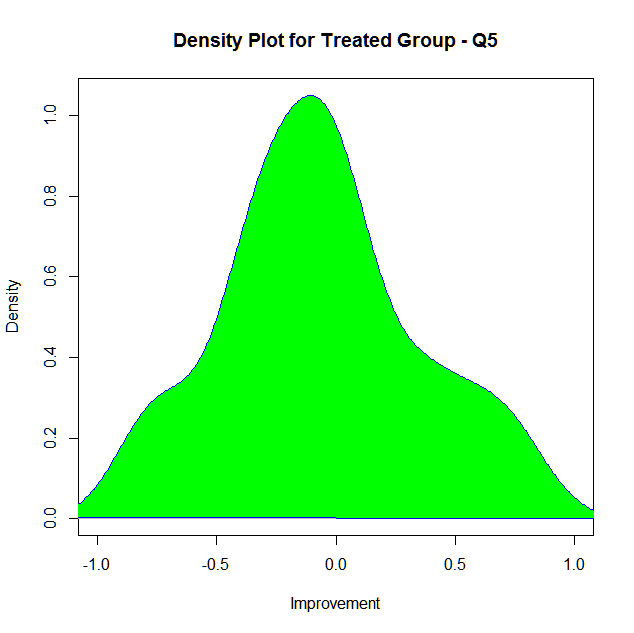
\includegraphics[width=1\linewidth]{figures/Imp_Treated-q5}
		\caption{IMP$_{(t_5)}$}
		\label{fig:Imp_Treated-q5}
	\end{minipage}
\end{figure}

\paragraph{Data Analysis}
After calculating the improvements i.e., \textit{IMP$_{(c_i)}$} and \textit{IMP$_{(t_i)}$} for each question, I used density plots to show their distribution. Figures~\ref{fig:Imp_Control-q1}, \ref{fig:Imp_Treated-q1}, \ref{fig:Imp_Control-q2}, \ref{fig:Imp_Treated-q2}, \ref{fig:Imp_Control-q3}, \ref{fig:Imp_Treated-q3}, \ref{fig:Imp_Control-q4}, \ref{fig:Imp_Treated-q4}, \ref{fig:Imp_Control-q5}, and \ref{fig:Imp_Treated-q5} show the density plots of the improvements for the control group and the treated group separately for each question. In the plots, the x-axis represents the improvement as described in Section \ref{subsubsec:evaluation_formula} ranging between -1 ("absolute negative learning") to 1 ("absolute positive learning"). The y-axis represents the density of 21 students in case of the control group and 18 students in case of the treated group lying over the interval.
These density plots show that the improvement values are scattered over the entire interval quite uniformly on both sides of the value 0. But, it is very difficult to say whether the values are more on the positive side or more on the negative side. So it's very hard to accept or reject the null hypothesis just by looking at these plots.

To gain an even better understanding of the data, I have further analyzed it with a t-test. As this hypothesis is related to one set of improvement data at a time i.e., either the improvement of the control group or the improvement of the treated group, I have used the one-sample t-test.   

The improvement is always calculated for posttest compared to the pretest. Here also improvement for control group is calculated subtracting control group pretest (\textit{RES$_{pre(c_i)}$}) results from control group posttest (\textit{RES$_{post(c_i)}$}) results and then dividing it by two for normalizing it between -1 to 1. Similarly, improvement for treated group is calculated subtracting treated group pretest (\textit{RES$_{pre(t_i)}$}) results from treated group posttest (\textit{RES$_{post(t_i)}$}) results and then dividing it by two for normalizing it between -1 to 1. Hence, the value less than 0 signifies "negative" improvement and the value greater than 0 signifies "positive" improvement. As two independent groups are involved, this hypothesis can be expressed as:   

Null Hypothesis, {H$_{NU2}$}: 
Mean (\textit{IMP$_{(c_i)}$}) < 0 and Mean (\textit{IMP$_{(t_i)}$}) < 0

Hence, I have included the option (\textit{alternative="greater"}) during the calculation which signifies that according to the operational hypothesis the mean values has to be greater than the default value 0. The results from the t-test are shown in Table~\ref{tab:t-test_Imp-control} and \ref{tab:t-test_Imp-treated} for control and treated group respectively. The 95\% confidence interval has been included for this t-test.

\paragraph{Discussion}
From the t-test results as shown in Table~\ref{tab:t-test_Imp-control}, it can be seen that the mean value of \textit{IMP$_{(c_i)}$} for all the questions are either less than 0 or close to 0.
Similarly, from the t-test results as shown in Table~\ref{tab:t-test_Imp-treated}, it can be seen that the mean values of \textit{IMP$_{(t_i)}$} for all the questions are either less than 0 or close to 0. But, the p-values in these cases are on higher side. 

This result indicates that participants learned negatively after using demon-bx tool. 
Some improvement can be seen for the treated group compared to the control group in terms of mean values, which indicates that demon-bx tool is more harmful without carefully designed scenarios (guidance steps for the user). With these results and higher p-values, the data were not significant enough to reject the null hypothesis {H$_{NU2}$}. This shows that for the fact whether demon-bx has a positive effect on the achievement of corresponding learning goals, no conclusive or significant results were obtained.

\begin{table}[ht]
	\centering	
	\begin{tabular}{|p{1cm}|p{1.5cm}|p{4.5cm}|p{1.5cm}|p{1.5cm}|p{1.5cm}|}
		\hline
		\rowcolor[gray]{.8}	
		\textbf{} & \textbf{Students} & \textbf{Factor} & \textbf{t-value} & \textbf{p-value} & \textbf{mean}\\
		\hline
		Q1 & 21 & improvement (control) &  -1.7589 & 0.9531 & -0.1904\\
		\hline
		Q2 & 21 & improvement (control) & 0.3841 & 0.3524 & 0.0357\\
		\hline
		Q3 & 21 & improvement (control) & -0.9604 & 0.8259 & -0.8928\\
		\hline	
		Q4 & 21 & improvement (control) & 0.2071 & 0.419 & 0.0238\\
		\hline
		Q5 & 21 & improvement (control) & -0.7853 & 0.7793 & -0.8333\\
		\hline			
	\end{tabular}
	\caption{t-test result showing Improvement (Control Group)}
	\label{tab:t-test_Imp-control}
\end{table}

\begin{table}[ht]
	\centering	
	\begin{tabular}{|p{1cm}|p{1.5cm}|p{4.5cm}|p{1.5cm}|p{1.5cm}|p{1.5cm}|}
		\hline
		\rowcolor[gray]{.8}	
		\textbf{} & \textbf{Students} & \textbf{Factor} & \textbf{t-value} & \textbf{p-value} & \textbf{mean}\\
		\hline
		Q1 & 18 & improvement (treated) &  -1.5226 & 0.9269 & -0.125\\
		\hline
		Q2 & 18 & improvement (treated) & -2.3739 & 0.9852 & -0.1527\\
		\hline
		Q3 & 18 & improvement (treated) & -0.9578 & 0.5376 & -0.0069\\
		\hline	
		Q4 & 18 & improvement (treated) & 0.8911 & 0.1927 & 0.0486\\
		\hline
		Q5 & 18 & improvement (treated) & -0.6439 & 0.7359 & -0.0625\\
		\hline			
	\end{tabular}
	\caption{t-test result showing Improvement (Treated Group)}
	\label{tab:t-test_Imp-treated}
\end{table}

\subsubsection{Analyzing Hypothesis 3}\label{subsubsec:hypothesis3}
Hypothesis 3 i.e., \textbf{H$_{OP3}$} and \textbf{H$_{NU3}$} is designed to investigate research question \textbf{RQ 4.2}. This hypothesis deals with the fact whether using demon-bx together with suitable scenarios is more effective than without scenarios. Data for \textbf{RQ 4.2} can be collected by comparing the improvement of the treated group than the control group. Because before appearing in the posttest, the treated group had used demon-bx with scenarios and the control group had used demon-bx without scenarios.

As five questions were asked, the improvement can be calculated for each question from the pretest and the posttest data separately for control and treated group.  

\paragraph{Data Analysis}
After calculating the improvements for control and treated group separately i.e., \textit{IMP$_{(c_i)}$} and \textit{IMP$_{(t_i)}$} for each question, I used density plots to show their distribution. Figures~\ref{fig:Imp_Control-q1}, \ref{fig:Imp_Treated-q1}, \ref{fig:Imp_Control-q2}, \ref{fig:Imp_Treated-q2}, \ref{fig:Imp_Control-q3}, \ref{fig:Imp_Treated-q3}, \ref{fig:Imp_Control-q4}, \ref{fig:Imp_Treated-q4}, \ref{fig:Imp_Control-q5}, and \ref{fig:Imp_Treated-q5} show the question wise density plots of the improvements for control and treated group. In the plots, the x-axis represents the improvement as described in Section \ref{subsubsec:evaluation_formula} ranging between -1 ("absolute negative learning") to 1 ("absolute positive learning"). The y-axis represents the density of 21 students in case of the control group and 18 students in case of the treated group lying over the interval. These figures show a comparison between the scattering of the improvement values for control and treated group. From these figures, both uniform and non-uniform distribution of the values can be seen on both sides of the value 0. But, for the naked eye, it is impossible to say whether the improvement in the case of treated group is more or the improvement in the case of the control group is more. So it's very hard to accept or reject the null hypothesis just by comparing these plots.

To gain a better understanding of the data, I have further analyzed it with a t-test. As this hypothesis is related to two sets of improvement data i.e., control and treated group, I have used the unpaired two-sample t-test.   

As mentioned earlier, improvement is always calculated for posttest compared to the pretest. Here also improvement for control group is calculated subtracting control group pretest (\textit{RES$_{pre(c_i)}$}) results from control group posttest (\textit{RES$_{post(c_i)}$}) results and then dividing it by two for normalizing it between -1 to 1. Similarly, improvement for treated group is calculated subtracting treated group pretest (\textit{RES$_{pre(t_i)}$}) results from treated group posttest (\textit{RES$_{post(t_i)}$}) results and then dividing it by two for normalizing it between -1 to 1. Hence, the value less than 0 signifies "negative" improvement and the value greater than 0 signifies "positive" improvement. As two independent groups are involved, this hypothesis can be expressed as:   

Null Hypothesis, {H$_{NU3}$}: Mean (\textit{IMP$_{(c_i)}$}) - Mean (\textit{IMP$_{(t_i)}$}) > 0

Hence, I have included the option (\textit{alternative="less", var.equal=TRUE}) during the calculation which signifies that according to the operational hypothesis, the mean value of the control group's improvement has to be less than the treated group's improvement assuming that both groups have equal standard deviation. Here I have assumed both groups to be equal as all the students were Master students from computer science branch with no or very less prior experience in synchronization, bidirectional transformation. The 95\% confidence interval has been included for this t-test. The results from the t-test for all the participants are shown in Table~\ref{tab:t-test_controltreated}. For this hypothesis, I have additionally calculated the results with the same t-test only for the good students, i.e., students with some bx background knowledge and more than 90\% marks in exams. The results from the t-test for the good students are shown in Table~\ref{tab:t-test_controltreated_good}.

\paragraph{Discussion}
From the t-test results (all participants) as shown in Table~\ref{tab:t-test_controltreated}, it can be seen that the mean difference of \textit{IMP$_{(c_i)}$} from \textit{IMP$_{(t_i)}$} for question Q2 is higher than 0 but for questions Q1, Q3, Q4, and Q5 are less than 0 with higher p-values. From the t-test results (good students) as shown in Table~\ref{tab:t-test_controltreated_good}, it can be seen that the mean difference of \textit{IMP$_{(c_i)}$} from \textit{IMP$_{(t_i)}$} for all questions are either less than 0 or very close to 0 with varying range of p-values.

These results indicate that some positive effect can be seen for the treated group compared to the control group and this improvement in the case of the good students are even better. But, with varying or higher p-values, the data were not significant enough to reject the null hypothesis {H$_{NU3}$}. This might be because of the fact that the scenarios are not designed for all types of audience. For example, good students or the students with prior knowledge about bx might comprehend the scenarios better than the average students or the students with no prior knowledge about bx. This shows that with suitable scenarios some positive learning can be achieved, but this is not evident in all cases and I was not able to conclude this with statistical significance.

\begin{table}[ht]
	\centering	
	\begin{tabular}{|p{1cm}|p{2cm}|p{3.5cm}|p{1.5cm}|p{1.5cm}|p{1.5cm}|}
		\hline
		\rowcolor[gray]{.8}	
		\textbf{} & \textbf{Students} & \textbf{Factor} & \textbf{t-value} & \textbf{p-value} & \textbf{mean diff.}\\
		\hline
		Q1 & 39 & Control vs. Treated & -0.8672 & 0.1957 & -0.0654\\
		\hline
		Q2 & 39 & Control vs. Treated & 1.6131 & 0.9424 & 0.1884\\
		\hline
		Q3 & 39 & Control vs. Treated & -0.6813 & 0.25 & -0.0823\\
		\hline	
		Q4 & 39 & Control vs. Treated & -0.1847 & 0.4272 & -0.0248\\
		\hline
		Q5 & 39 & Control vs. Treated & -0.143 & 0.4435 & -0.0208\\
		\hline			
	\end{tabular}
	\caption{t-test result showing Improvement (Control vs. Treated Group: All Participants)}
	\label{tab:t-test_controltreated}
\end{table}

\begin{table}[ht]
	\centering	
	\begin{tabular}{|p{1cm}|p{2cm}|p{3.5cm}|p{1.5cm}|p{1.5cm}|p{1.5cm}|}
		\hline
		\rowcolor[gray]{.8}	
		\textbf{} & \textbf{Good Students} & \textbf{Factor} & \textbf{t-value} & \textbf{p-value} & \textbf{mean diff.}\\
		\hline
		Q1 & 12 & Control vs. Treated & -2.4058 & 0.0184 & -0.4791\\
		\hline
		Q2 & 12 & Control vs. Treated & -1.7341 & 0.0567 & -0.2708\\
		\hline
		Q3 & 12 & Control vs. Treated & -1.2738 & 0.1158 & -0.2916\\
		\hline	
		Q4 & 12 & Control vs. Treated & -0.584 & 0.2861 & -0.1666\\
		\hline
		Q5 & 12 & Control vs. Treated & 0.3274 & 0.625 & 0.0833\\
		\hline			
	\end{tabular}
	\caption{t-test result showing Improvement (Control vs. Treated Group: Good Students)}
	\label{tab:t-test_controltreated_good}
\end{table}
